% SPDX-License-Identifier: CC0-1.0
\documentclass[11pt,a4paper]{article}
\usepackage[T1]{fontenc}
\usepackage[utf8]{inputenc}
\usepackage{lmodern}
\usepackage[margin=2.35cm,headheight=14pt]{geometry}
\usepackage{amsmath,amssymb,amsthm,mathtools}
\usepackage{microtype,booktabs,longtable,array,multicol}
\usepackage[dvipsnames]{xcolor}
\usepackage{enumitem,titlesec,fancyhdr}
\usepackage{tikz}
\usetikzlibrary{positioning,calc}
\usepackage{listings}
\usepackage[colorlinks=true,linkcolor=MidnightBlue,citecolor=MidnightBlue,
  urlcolor=MidnightBlue]{hyperref}
\definecolor{Ink}{HTML}{16324F}
\definecolor{Accent}{HTML}{4E5C3D}
\definecolor{Pale}{HTML}{F2F5F7}
\titleformat{\section}{\Large\bfseries\color{Ink}}{\thesection}{0.7em}{}
\titleformat{\subsection}{\large\bfseries\color{Accent}}{\thesubsection}{0.7em}{}
\pagestyle{fancy}
\fancyhf{}
\fancyhead[L]{\small\color{Ink}A sharp cover bound for lattice congruences}
\fancyhead[R]{\small Research draft}
\fancyfoot[C]{\thepage}
\renewcommand{\headrulewidth}{0.3pt}
\setlength{\parskip}{0.35em}
\setlength{\parindent}{1.25em}
\setlength{\emergencystretch}{2em}
\setlist{itemsep=0.15em,topsep=0.3em}
\allowdisplaybreaks[2]
\numberwithin{equation}{section}
\newtheorem{theorem}{Theorem}[section]
\newtheorem{lemma}[theorem]{Lemma}
\newtheorem{corollary}[theorem]{Corollary}
\newtheorem{proposition}[theorem]{Proposition}
\theoremstyle{definition}
\newtheorem{definition}[theorem]{Definition}
\newtheorem{example}[theorem]{Example}
\theoremstyle{remark}
\newtheorem{remark}[theorem]{Remark}
\DeclareMathOperator{\Con}{Con}
\DeclareMathOperator{\con}{con}
\DeclareMathOperator{\Ji}{Ji}
\DeclareMathOperator{\Jr}{Jr}
\DeclareMathOperator{\Mr}{Mr}
\DeclareMathOperator{\Idl}{Idl}
\DeclareMathOperator{\Skel}{Skel}
\DeclareMathOperator{\UpCov}{UpCov}
\DeclareMathOperator{\LoCov}{LoCov}
\DeclareMathOperator{\cdens}{cd}
\newcommand{\glue}{\mathbin{\dotplus}}
\newcommand{\N}{\mathbb N}
\newcommand{\Q}{\mathbb Q}
\newcommand{\R}{\mathbb R}
\newcommand{\eqcon}{\mathbf 0_L}
\newcommand{\allcon}{\mathbf 1_L}
\newcommand{\set}[1]{\{#1\}}
\newcommand{\card}[1]{\lvert #1\rvert}
\lstset{basicstyle=\small\ttfamily,columns=fullflexible,keepspaces=true,
  frame=single,rulecolor=\color{black!20},backgroundcolor=\color{Pale},
  breaklines=true,showstringspaces=false,aboveskip=0.7em,belowskip=0.7em}
\hypersetup{pdftitle={A sharp cover bound for congruences of finite lattices},
  pdfauthor={AI-assisted research draft},
  pdfsubject={Czedli's k-cover suggestion, equality cases, a sharp gap, and skeleton bounds}}
\title{\vspace{-1.0em}\LARGE\bfseries\color{Ink}
A sharp cover bound for congruences\nobreak\\[0.2em] of finite lattices\\[0.6em]
\large\normalfont\color{Accent}Pairwise joins, equality, and bounded skeletons}
\author{AI-assisted research draft}
\date{20 September 2026}

\begin{document}
\maketitle
\thispagestyle{empty}
\begin{abstract}
Let $L$ be a finite lattice with $n$ elements. We give an elementary proof that,
if one element has at least $k$ upper covers and $k\ge3$, then
$\card{\Con(L)}\le 2^{n-k-1}$. This supplies the strengthening suggested immediately
after Lemma~4.4 of Cz\'edli's \emph{Accumulation points of congruence densities of
finite lattices}, replacing its multicolor Ramsey threshold by $k$ itself.
The proof counts two complementary losses: join-reducible elements and repeated
principal-congruence labels. Equalities between pairwise joins control both losses.
We also characterize equality: precisely a length-two lattice with $k$ atoms,
with an arbitrary chain attached at either end. Among nonextremal lattices with
such a cover configuration, the sharp next bound is
$3\cdot 2^{n-k-3}$. Finally, for $\cdens(L)\ge p>0$ and
$t=\lfloor\log_2(1/p)\rfloor$, the skeleton introduced by Cz\'edli has at most
$2t(\max\{2,t\}+1)$ elements. All necessary congruence tools are proved here.
Exact exhaustive tests cover every isomorphism class through eight elements,
represented by 4,008 naturally labelled lattices, and check 6,292 cover
configurations. The archive contains the programs and their recorded output.
\end{abstract}

\medskip
\noindent\colorbox{Pale}{\parbox{\dimexpr\linewidth-2\fboxsep\relax}{%
\small\textbf{Status.} This is a proposed research solution with complete written
proofs, not an independently refereed or proof-assistant-verified result.
The literature search found the stated question unresolved in the consulted
sources; it does not certify priority. The elementary background, the source's
existing special cases, and the contributions of this draft are distinguished
below.}}

\medskip
\noindent\textbf{Keywords.} Finite lattice; lattice congruence; upper cover;
join-irreducible element; congruence density; extremal lattice; skeleton.

\noindent\textbf{Selection record.} A single operating-system random draw from
80 mathematical areas selected number~10, \emph{lattice theory}. No redraw was
made. The complete list and the exclusion audit are included in the package.

\clearpage
\tableofcontents
\clearpage

\section{The question and the results}
\subsection{A precise published target}
A \emph{lattice} is a partially ordered set in which any two elements $x,y$ have
a greatest lower bound $x\wedge y$ and a least upper bound $x\vee y$.
An element $a$ \emph{covers} $u$, written $u\prec a$, when $u<a$ and no element
lies strictly between them. Throughout, lattices are finite and nonempty.
A \emph{congruence} is an equivalence relation compatible with both lattice
operations. We write $\Con(L)$ for the set of congruences of $L$.

The normalization
\begin{equation}\label{eq:density}
  \cdens(L)=\frac{\card{\Con(L)}}{2^{\card L-1}}
\end{equation}
is the congruence density used by Cz\'edli. The denominator is the classical
maximum for a lattice of that size, attributed to Freese~\cite{freese}; a
self-contained proof appears in Section~\ref{sec:tools}.

For $k\ge3$, let $R_{k-1}(k)=R(k,\ldots,k)$ be the Ramsey number with $k-1$
colors. Cz\'edli proves that $R_{k-1}(k)$ upper covers of one element force
$\cdens(L)\le2^{-k}$, and immediately suggests that $k$ upper covers might
already suffice~\cite[Lemma~4.4 and the following sentence, p.~8]{czedli}.
The precise target of this article is therefore
\begin{equation}\label{eq:target}
 k\ge3,\quad \card{\UpCov_L(u)}\ge k
 \quad\Longrightarrow\quad \cdens(L)\le2^{-k}.
\end{equation}
This is an informal suggestion in the source, not a numbered conjecture.
We occasionally call it the \emph{$k$-cover question} as a local shorthand.
In particular, this article is not about covering systems of integers, geometric
lattices of Euclidean space, or the much broader congruence-lattice representation
problem.

\subsection{The sharp theorem}
Let $C_s$ denote the chain with $s$ elements, including $C_1$.
Let $M_k$ consist of a bottom $u$, a top $v$, and $k$ pairwise incomparable
intermediate elements $a_1,\ldots,a_k$. Thus $\card{M_k}=k+2$.
The \emph{glued sum} $A\glue B$ identifies the top of $A$ with the bottom of $B$
and puts every element of $A$ below every element of $B$.

\begin{theorem}[Sharp cover bound and all equality cases]\label{thm:main}
Let $k\ge3$, and let $L$ be an $n$-element lattice with an element having at least
$k$ upper covers. Then
\begin{equation}\label{eq:main}
 \card{\Con(L)}\le2^{n-k-1}.
\end{equation}
Equality holds if and only if
\begin{equation}\label{eq:extremal}
 L\cong C_s\glue M_k\glue C_t
 \qquad(s,t\ge1,\quad s+t=n-k).
\end{equation}
The same statements hold with ``lower covers'' in place of ``upper covers''.
For every $n\ge k+2$, the bound is attained.
\end{theorem}

The proof of the inequality is in Section~\ref{sec:bound}; the equality analysis
is in Section~\ref{sec:equality}. The proof does not assume modularity,
semimodularity, distributivity of $L$, or that $u$ is the bottom element.
Nor does it require the upper covers to have a common pairwise join.
The latter condition is the special case already covered by
Cz\'edli's Lemma~4.3~\cite{czedli}.

There is also a sharp gap. If $L$ is not of the form~\eqref{eq:extremal}, then
\begin{equation}\label{eq:gap-intro}
 \cdens(L)\le\frac34\,2^{-k}.
\end{equation}
For every $n\ge k+3$, this is attained among $n$-element lattices with $k$ upper
covers. Section~\ref{sec:gap} proves this assertion; it determines the second
largest value in the cover-constrained class, but does not classify all of its
witnesses.

\subsection{Selection, source status, and attribution}
The attached manifest~\cite{manifest} was read in full and treated as an exclusion
list. No listed problem concerns the finite-lattice congruence bound considered
here. The random draw was performed before selecting this question; the selected
area was retained throughout. Appendix~\ref{app:selection} records the method
and the 80-area list.

As checked on 20~September~2026, arXiv listed only version~1 of the target paper,
dated 12~March~2026. The author's publication list reports its acceptance by
\emph{CUBO} on 14~August~2026 and still dates the linked manuscript
12~March~2026~\cite{publist}. Searches for the exact title and for the cover
suggestion did not locate a subsequent resolution. This is evidence for selecting
the problem, not an exhaustive priority determination.

In particular, the $k=3$ density range overlaps earlier classification work:
Cz\'edli's separate paper describes all lattices with density exceeding
$3/32$~\cite{czedli332}. No claim is made that every low-parameter consequence
below was previously unknown. The contributions proposed here are the uniform
all-$k$ proof, its equality argument, the resulting cover-constrained extremal
statements, and the quadratic skeleton estimate. The finite congruence theory
used to obtain them is classical and is reproved, not claimed as new.

\section{Elementary congruence tools}\label{sec:tools}
\subsection{Irreducible elements and principal congruences}
Every finite lattice has a bottom $0$ and a top $1$.
Write $\Ji(L)$ for the set of elements having exactly one lower cover.
For $j\in\Ji(L)$, denote that lower cover by $j_*$. Write $\Jr(L)$ for the
elements having at least two lower covers, and $\Mr(L)$ for those having at
least two upper covers. Thus, with $n=\card L$ and $m=\card{\Jr(L)}$,
\begin{equation}\label{eq:partition-elements}
 L=\{0\}\mathbin{\dot\cup}\Ji(L)\mathbin{\dot\cup}\Jr(L),
 \qquad \card{\Ji(L)}=n-1-m.
\end{equation}

These are also the familiar algebraic notions. A nonzero element is
join-irreducible precisely when it cannot be expressed as a join of two strictly
smaller elements. Indeed, a unique lower cover lies above every strictly smaller
element. Conversely, two distinct lower covers have join equal to the element
they cover. In particular, the join of two incomparable elements belongs to
$\Jr(L)$; the dual assertion holds for their meet.

For $x,y\in L$, let $\con(x,y)$ be the least congruence identifying $x$ and $y$.
It exists as the intersection of all such congruences. Congruences are ordered
by inclusion as binary relations. Their least and greatest elements are the
equality relation $\eqcon$ and the universal relation $\allcon$.

\begin{lemma}[Convexity of classes]\label{lem:convex}
Every congruence class in a finite lattice is an interval. In particular, if
$x\le z\le y$ and $x\equiv y\pmod\theta$, then $x\equiv z\equiv y\pmod\theta$.
\end{lemma}
\begin{proof}
Apply meet with $z$ to $x\equiv y$: it gives $x\equiv z$.
A congruence class is closed under finite meets and joins, so it has a least and
a greatest element. Convexity then identifies it with the interval between them.
\end{proof}

\begin{lemma}[Transposition without a cover hypothesis]\label{lem:transpose}
For all $x,y\in L$,
\begin{equation}\label{eq:transpose}
 \con(x\wedge y,x)=\con(y,x\vee y).
\end{equation}
\end{lemma}
\begin{proof}
Joining a pair $x\wedge y\equiv x$ with $y$ gives $y\equiv x\vee y$.
Conversely, meeting $y\equiv x\vee y$ with $x$ gives $x\wedge y\equiv x$.
Each principal congruence is therefore contained in the other.
\end{proof}

\begin{lemma}[A join-irreducible representative for every edge]\label{lem:representative}
If $x\prec y$, there is $j\in\Ji(L)$ such that
\begin{equation}\label{eq:representative}
 j\vee x=y,\qquad j\wedge x=j_*,\qquad
 \con(x,y)=\con(j_*,j).
\end{equation}
If $a_1,\ldots,a_k$ are distinct upper covers of the same $u$, the representatives
$j_1,\ldots,j_k$ obtained in this way are distinct.
\end{lemma}
\begin{proof}
Choose $j$ minimal in $\downarrow y\setminus\downarrow x$.
Then $j\ne0$, and every element strictly below $j$ lies below $x$.
If $j$ had two distinct lower covers, their join would be $j$, forcing $j\le x$.
Thus $j\in\Ji(L)$ and $j_*\le x$.
The inequalities $j\nleq x$ and $j\le y$ imply $x<j\vee x\le y$;
the cover hypothesis gives $j\vee x=y$.
Also $j\wedge x<j$, so $j\wedge x\le j_*$, while $j_*\le j\wedge x$.
Equation~\eqref{eq:transpose} proves the congruence equality.
For the final assertion, $j_i=j_h$ would imply
$a_i=j_i\vee u=j_h\vee u=a_h$.
\end{proof}

\subsection{Signatures and the classical counting bound}
Assign to each $j\in\Ji(L)$ the label
\begin{equation}\label{eq:labels}
 \gamma_j=\con(j_*,j),\qquad
 Q(L)=\{\gamma_j:j\in\Ji(L)\},\qquad q=\card{Q(L)}.
\end{equation}
The set $Q(L)$ contains \emph{distinct congruences}: repetitions among the
$\gamma_j$ have been removed. It is a poset under inclusion.
For $\theta\in\Con(L)$, define its signature
\begin{equation}\label{eq:signature}
 \Sigma(\theta)=\{\gamma\in Q(L):\gamma\le\theta\}.
\end{equation}

\begin{lemma}[Signatures determine congruences]\label{lem:signature}
The map $\Sigma$ is injective. Consequently
\begin{equation}\label{eq:classical}
 \card{\Con(L)}\le2^q\le2^{\card{\Ji(L)}}
   =2^{n-1-m}\le2^{n-1}.
\end{equation}
Moreover, every congruence is the join of the principal labels that it contains.
\end{lemma}
\begin{proof}
A congruence is determined by the cover edges it collapses.
For comparable $x\le y$, the relation $x\equiv y$ holds exactly when all edges
of a saturated chain from $x$ to $y$ collapse; use
Lemma~\ref{lem:convex} for one direction and transitivity for the other.
For arbitrary $x,y$, the relation is equivalent to both
$x\equiv x\wedge y$ and $y\equiv x\wedge y$.
Lemma~\ref{lem:representative} expresses the principal congruence of each edge
as one of the $\gamma_j$. Thus its collapse is determined by~\eqref{eq:signature}.
This proves injectivity and the cardinality bounds.

Let $\rho$ be the join of all $\gamma\in\Sigma(\theta)$.
Then $\rho\le\theta$, and every edge collapsed by $\theta$ is also collapsed by
$\rho$. The preceding argument gives $\rho=\theta$.
\end{proof}

An $s$-element chain has exactly $2^{s-1}$ congruences: choose an arbitrary subset
of its $s-1$ adjacent edges to collapse. The resulting blocks are intervals,
and interval partitions are compatible with minimum and maximum.
This verifies that the denominator in~\eqref{eq:density} really is the maximum.

For the main inequality, injectivity alone is enough. We also give the stronger
classical description because it yields a sharp gap and clarifies equality.
An \emph{order ideal} of a poset is a downward-closed subset, with the empty set
included.

\begin{lemma}[Prime edge labels and ideal representation]\label{lem:ideals}
For an edge $x\prec y$, its principal congruence is join-prime: if
$\con(x,y)\le\theta\vee\phi$, then it is contained in $\theta$ or in $\phi$.
Furthermore,
\begin{equation}\label{eq:ideal-representation}
 \Sigma:\Con(L)\longrightarrow\Idl(Q(L))
 \quad\text{is a bijection}.
\end{equation}
In particular, $\card{\Con(L)}=2^q$ if and only if $Q(L)$ is an antichain.
\end{lemma}
\begin{proof}
The join of two congruences is the equivalence closure of their union.
To see compatibility of this closure, apply a lattice operation with one argument
fixed to a connecting walk; each step remains in the congruence responsible for
that step. Compatibility in both arguments follows by changing one at a time.
Thus $x\equiv y\pmod{\theta\vee\phi}$ gives a walk from $x$ to $y$ whose steps
belong to $\theta$ or to $\phi$.

Apply the unary lattice polynomial $z\mapsto(z\vee x)\wedge y$ to the walk.
Its image lies in $[x,y]=\{x,y\}$, and its endpoints remain $x,y$.
At least one step changes from one endpoint to the other. That step witnesses
$x\equiv y$ in $\theta$ or in $\phi$. This proves join-primeness.

Every signature is an ideal. Conversely, for an ideal $I\subseteq Q(L)$, put
$\theta=\bigvee I$, using $\eqcon$ for the empty join.
Each $\gamma\in Q(L)$ is an edge label, so finite join-primeness implies that
$\gamma\le\bigvee I$ exactly when $\gamma\le\delta$ for some $\delta\in I$.
Since $I$ is downward closed, this is equivalent to $\gamma\in I$.
Therefore $\Sigma(\theta)=I$, proving surjectivity. Injectivity is
Lemma~\ref{lem:signature}.
Finally, all $2^q$ subsets of a finite poset are ideals exactly when it has no
comparability between distinct elements.
\end{proof}

\section{Pairwise joins and the cover bound}\label{sec:bound}
\subsection{A local cover configuration}
Fix $u\in L$ and $k\ge3$ distinct upper covers $a_1,\ldots,a_k$ of $u$.
We call the selected configuration a \emph{fan}; the selection need not contain
all upper covers of $u$. Put
\begin{equation}\label{eq:fan-data}
 \alpha_i=\con(u,a_i),\qquad
 r=\card{\{\alpha_1,\ldots,\alpha_k\}},\qquad
 H=\{a_i\vee a_j:1\le i<j\le k\}.
\end{equation}
Distinct upper covers are incomparable and have meet $u$. Therefore
\begin{equation}\label{eq:pair-data}
 a_i\wedge a_j=u,\qquad H\subseteq\Jr(L),\qquad
 \alpha_i=\con(a_j,a_i\vee a_j)\quad(i\ne j).
\end{equation}
The last equality is transposition. Notice that
$[a_j,a_i\vee a_j]$ need not be a cover interval. That is why the unrestricted
form of Lemma~\ref{lem:transpose} is useful.

\begin{lemma}[A third cover below a pairwise join]\label{lem:support}
For distinct $i,j,h$, if $a_h\le a_i\vee a_j$, then
\begin{equation}\label{eq:support}
 \alpha_h\le\alpha_i\quad\text{and}\quad\alpha_h\le\alpha_j.
\end{equation}
\end{lemma}
\begin{proof}
The relation $a_j\equiv a_i\vee a_j\pmod{\alpha_i}$, met with $a_h$, gives
$u\equiv a_h\pmod{\alpha_i}$. Interchange $i,j$ for the other inclusion.
\end{proof}

\begin{lemma}[Join collisions]\label{lem:collision}
The following statements hold for a fan.
\begin{enumerate}[label=\textup{(\roman*)}]
\item If $i,j,h$ are distinct and $a_i\vee a_j=a_i\vee a_h$, then
\begin{equation}\label{eq:incident-collision}
 \alpha_j=\alpha_h\le\alpha_i.
\end{equation}
\item If $i,j,h,\ell$ are distinct and
$a_i\vee a_j=a_h\vee a_\ell$, then all four labels
$\alpha_i,\alpha_j,\alpha_h,\alpha_\ell$ are equal.
\end{enumerate}
\end{lemma}
\begin{proof}
For (i), write the common join as $v$. Transposing against $a_i$ gives
$\alpha_j=\con(a_i,v)=\alpha_h$.
Since $a_h\le a_i\vee a_j$, Lemma~\ref{lem:support} gives
$\alpha_h\le\alpha_i$.

For (ii), each of $a_h,a_\ell$ lies below $a_i\vee a_j$, so its label is
contained in both $\alpha_i$ and $\alpha_j$. Conversely, each of $a_i,a_j$
lies below $a_h\vee a_\ell$, so its label is contained in both
$\alpha_h$ and $\alpha_\ell$. These inclusions give the assertion.
\end{proof}

The combinatorial point is that distinct congruence labels prevent collisions
among the corresponding pairwise joins. This is more informative than treating
pairwise joins as unrelated colors in an arbitrary complete-graph coloring.

\subsection{The two losses in the exponent}
\begin{lemma}[The join-reducible budget]\label{lem:budget}
For a fan of $k\ge3$ upper covers with $r$ distinct labels,
\begin{equation}\label{eq:budget}
 m=\card{\Jr(L)}\ge r.
\end{equation}
More precisely,
\begin{equation}\label{eq:phi}
 m\ge\varphi(r),\qquad
 \varphi(r)=
 \begin{cases}
 1,&r=1,\\
 2,&r=2,\\
 \binom r2,&r\ge3.
 \end{cases}
\end{equation}
\end{lemma}
\begin{proof}
For $r=1$, the nonempty set $H$ supplies a join-reducible element.
For $r=2$, there are two covers $a,b$ with one label and a cover $c$ with the
other: here the hypothesis $k\ge3$ is essential. If $a\vee b=a\vee c$,
Lemma~\ref{lem:collision}(i) would equate the two labels.
Thus these two joins are distinct members of $\Jr(L)$.

For $r\ge3$, select one cover from each label class.
The $\binom r2$ pairwise joins of these selected covers are all different.
Two incident pairs cannot have the same join by part~(i) of the collision lemma;
two disjoint pairs cannot have the same join by part~(ii).
All their joins belong to $\Jr(L)$.
Finally, $\binom r2\ge r$ when $r\ge3$.
\end{proof}

\begin{lemma}[The repeated-label budget]\label{lem:duplicates}
For the same fan,
\begin{equation}\label{eq:duplicates}
 q\le\card{\Ji(L)}-k+r=n-1-m-k+r.
\end{equation}
\end{lemma}
\begin{proof}
Lemma~\ref{lem:representative} supplies $k$ distinct elements
$j_1,\ldots,j_k$ of $\Ji(L)$ whose labels are $\alpha_1,\ldots,\alpha_k$.
They account for only $r$ distinct labels. Each of the other
$\card{\Ji(L)}-k$ elements can add at most one more.
\end{proof}

\begin{proof}[Proof of the inequality in Theorem~\ref{thm:main}]
Combine the signature bound with the two budgets:
\begin{align*}
 \card{\Con(L)}
 &\le2^q\\
 &\le2^{n-1-m-k+r}\\
 &\le2^{n-1-k}.
\end{align*}
The first loss is the $m$ elements that are not available as nonzero
join-irreducible generators. The second loss is the $k-r$ repetitions among
the fan's $k$ distinct representatives. Their total is
$m+(k-r)\ge k$.
A lattice and its order dual have exactly the same congruences, with meet and
join interchanged, so the lower-cover statement follows as well.
\end{proof}

\begin{corollary}[A label-sensitive exponent]\label{cor:exponent}
Under the fan hypotheses,
\begin{equation}\label{eq:refined-exponent}
 \cdens(L)\le2^{-m-k+r}\le2^{-k-\varphi(r)+r}.
\end{equation}
For example, four distinct fan labels give $\cdens(L)\le2^{-k-2}$,
and five distinct labels give $\cdens(L)\le2^{-k-5}$.
\end{corollary}

\section{Why equality forces a single diamond}\label{sec:equality}
The numerical proof also retains enough information to determine the lattice.
This requires distinguishing \emph{equal labels} from \emph{independent labels}:
even when the count of labels is optimal, comparabilities between them make some
subsets unavailable as signatures.

\begin{lemma}[Antichain labels strengthen the budget]\label{lem:antichain-budget}
Suppose $Q(L)$ is an antichain and the fan has $r\ge2$ distinct labels.
Then $\card{\Jr(L)}>r$.
\end{lemma}
\begin{proof}
For $r=2$, choose distinct covers $a,b$ with label $A$ and a cover $c$ with label
$B\ne A$. The joins $a\vee b$, $a\vee c$, and $b\vee c$ are all distinct.
The first cannot equal either of the other two, as that would give $A=B$.
Equality of the last two would give $A\le B$ by
Lemma~\ref{lem:collision}(i), contrary to the antichain assumption.
Thus $m\ge3>2$.

For $r\ge3$, choose $r$ covers with pairwise distinct labels.
Their $\binom r2$ pairwise joins are distinct, as before.
Let $w$ be the join of all the selected covers. It cannot equal any of those
pairwise joins: a third cover would lie below that pairwise join, and
Lemma~\ref{lem:support} would give a comparability between different labels.
Also $w\in\Jr(L)$. Indeed, if $w$ were join-irreducible, every selected cover,
being strictly smaller than $w$, would lie below its unique lower cover;
their join could not be $w$.
Hence $m\ge\binom r2+1>r$.
\end{proof}

\begin{lemma}[Congruences of a quotient]\label{lem:quotient}
For $\alpha\in\Con(L)$, congruences of $L/\alpha$ correspond bijectively to
congruences of $L$ containing $\alpha$.
\end{lemma}
\begin{proof}
Pull an equivalence relation on the quotient back along the quotient map.
Conversely, a congruence containing $\alpha$ induces a well-defined relation on
$\alpha$-classes. The two operations are inverse, and compatibility follows
because the quotient operations are induced by those of $L$.
\end{proof}

\begin{proof}[Proof of the equality characterization in Theorem~\ref{thm:main}]
Assume $\card{\Con(L)}=2^{n-k-1}$ and choose a fan of $k$ upper covers of $u$.
Every inequality in the numerical proof must be an equality. Therefore
\begin{equation}\label{eq:equality-budget}
 m=r,\qquad q=n-k-1,\qquad \card{\Con(L)}=2^q.
\end{equation}
By Lemma~\ref{lem:ideals}, $Q(L)$ is an antichain.
Lemma~\ref{lem:antichain-budget} rules out $r\ge2$, so
\begin{equation}\label{eq:one-reducible}
 r=m=1.
\end{equation}
Let $v$ be the unique join-reducible element, and let $\alpha$ be the common
label of the fan. Every pairwise join of its covers is $v$.
Consequently $\alpha$ identifies all elements of
\begin{equation}\label{eq:block}
 B=\{u,a_1,\ldots,a_k,v\}.
\end{equation}
In detail, it identifies each $a_i$ with $u$, and joining two of these
identifications also identifies $v$ with $u$.

We next show that $B$ is exactly the sole nonsingleton $\alpha$-class.
Since all subsets of $Q(L)$ occur as signatures, exactly $2^{q-1}$ congruences
contain $\alpha$. By Lemma~\ref{lem:quotient} and the classical bound applied
to $L/\alpha$,
\begin{equation}\label{eq:quotient-lower}
 2^{n-k-2}=2^{q-1}
   =\card{\Con(L/\alpha)}\le2^{\card{L/\alpha}-1}.
\end{equation}
Thus $\card{L/\alpha}\ge n-k-1$.
On the other hand, the $k+2$ distinct elements in~\eqref{eq:block} belong to a
single class, so $\card{L/\alpha}\le n-k-1$.
Equality follows. Merging $k+2$ elements already accounts for the full reduction
of $k+1$ in the quotient size; no additional element can enter that class and no
other class can be nonsingleton. Convexity now gives
\begin{equation}\label{eq:interval-diamond}
 [u,v]=B\cong M_k.
\end{equation}

It remains to locate every element outside this interval.
First, each $x\in L$ is comparable with $v$. Otherwise $x\vee v$ would be a
join-reducible element strictly greater than $v$, contradicting its uniqueness.
Second, if $x\le v$ and $x\notin B$, meet the relation $u\equiv v\pmod\alpha$
with $x$. This gives $u\wedge x\equiv x\pmod\alpha$.
The class of $x$ is a singleton, so $u\wedge x=x$, that is, $x\le u$.
Thus every element outside $B$ lies below $u$ or above $v$.

Both $[0,u]$ and $[v,1]$ are chains. Incomparable elements in the former would
have a join-reducible join at most $u<v$, and incomparable elements in the latter
would have a join-reducible join strictly above $v$. Both are impossible.
Consequently $L\cong C_s\glue M_k\glue C_t$ for some $s,t\ge1$, and counting
the two identified endpoints gives $n=s+(k+2)+t-2=k+s+t$.

Conversely, $M_k$ is simple when $k\ge3$.
Its lower-edge labels are all equal by
Lemma~\ref{lem:collision}(i), and that common label identifies the whole lattice.
Every upper-edge label equals a lower-edge label by transposition.
A nontrivial congruence collapses an edge by the argument in
Lemma~\ref{lem:signature}, so its only congruences are equality and universality.
Therefore $\card{\Con(M_k)}=2$.

Congruences of a glued sum $A\glue D$ are in bijection with pairs of congruences
of $A$ and $D$. Restrictions give one direction. In the other, retain all classes
except that the two classes containing the identified point are joined into one.
Equivalently, map the two summands to their respective quotient lattices and
glue the quotients at the image of the common point. This map is a lattice
homomorphism: within each summand it is a quotient map, and across summands
meet selects the lower argument while join selects the upper. Its kernel is
exactly the described partition, and its restrictions recover the original
congruences. These constructions are inverse.
It follows that
\begin{equation}\label{eq:glued-count}
 \card{\Con(C_s\glue M_k\glue C_t)}
 =2^{s-1}\cdot2\cdot2^{t-1}
 =2^{s+t-1}=2^{n-k-1}.
\end{equation}
Finally, order duality interchanges the two exterior chains and preserves $M_k$,
so the equality family is the same for lower covers.
\end{proof}

\begin{figure}[htbp]
\centering
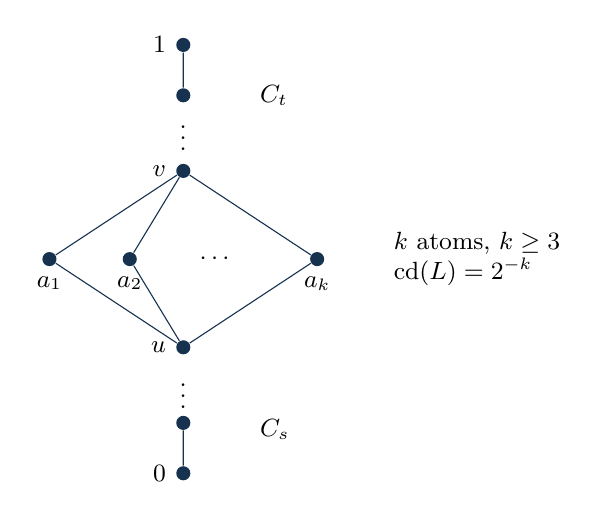
\begin{tikzpicture}[x=0.85cm,y=0.8cm,
  dot/.style={circle,fill=Ink,inner sep=1.8pt},every node/.style={font=\small}]
\node[dot,label=left:$0$] (b) at (0,0) {};
\node[dot] (b1) at (0,0.8) {};
\node (dotsb) at (0,1.35) {$\vdots$};
\node[dot,label=left:$u$] (u) at (0,2) {};
\node[dot,label=below:$a_1$] (a1) at (-2,3.4) {};
\node[dot,label=below:$a_2$] (a2) at (-0.8,3.4) {};
\node (dots) at (0.5,3.4) {$\cdots$};
\node[dot,label=below:$a_k$] (ak) at (2,3.4) {};
\node[dot,label=left:$v$] (v) at (0,4.8) {};
\node (dotst) at (0,5.45) {$\vdots$};
\node[dot] (t1) at (0,6) {};
\node[dot,label=left:$1$] (t) at (0,6.8) {};
\draw[Ink] (b)--(b1) (u)--(a1)--(v) (u)--(a2)--(v)
 (u)--(ak)--(v) (t1)--(t);
\node[align=left,anchor=west] at (3,3.4)
 {$k$ atoms, $k\ge3$\\$\cdens(L)=2^{-k}$};
\node[anchor=west] at (1,0.7) {$C_s$};
\node[anchor=west] at (1,6) {$C_t$};
\end{tikzpicture}
\caption{All equality cases. Either exterior chain may consist of its glued
endpoint alone. The omitted intermediate atoms have the same two incident edges
as the displayed atoms.}
\label{fig:extremal}
\end{figure}

\section{A sharp gap below the maximum}\label{sec:gap}
\begin{lemma}[A missing ideal costs at least one quarter]\label{lem:ideal-gap}
If a $q$-element poset $P$ is not an antichain, then
$\card{\Idl(P)}\le3\cdot2^{q-2}$.
\end{lemma}
\begin{proof}
Choose distinct $a<b$ in $P$. No ideal can contain $b$ while omitting $a$.
Exactly one of the four inclusion patterns on $\{a,b\}$ is therefore forbidden.
The remaining $q-2$ elements have at most $2^{q-2}$ patterns.
\end{proof}

\begin{theorem}[The second extremal value]\label{thm:gap}
Let $k\ge3$. If an $n$-element lattice $L$ has an element with at least $k$ upper
covers and is not of the form~\eqref{eq:extremal}, then $n\ge k+3$ and
\begin{equation}\label{eq:gap}
 \card{\Con(L)}\le3\cdot2^{n-k-3},\qquad
 \cdens(L)\le3\cdot2^{-k-2}.
\end{equation}
For every $n\ge k+3$, equality in this bound is attained.
\end{theorem}
\begin{proof}
Put $N=n-k-1$. Section~\ref{sec:bound} gives $q\le N$.
If $q\le N-1$, then $\card{\Con(L)}\le2^{N-1}\le3\cdot2^{N-2}$.
If $q=N$, nonextremality and Lemma~\ref{lem:ideals} imply that $Q(L)$ is not an
antichain. Lemma~\ref{lem:ideal-gap} gives the same bound.
The case $N=1$ admits no nonextremal lattice: every nonsingleton lattice has at
least two congruences, which is already the maximum in that case.

For sharpness, form $T_k$ by adding one new element $z$ to $M_k$ on the edge
$a_1\prec v$, replacing it by $a_1\prec z\prec v$.
The $k$ lower edges remain covers and all their labels are the universal
congruence, as all pairwise joins are still $v$.
The join-irreducibles are $a_1,\ldots,a_k,z$.
The remaining label $\beta=\con(a_1,z)$ has exactly one nonsingleton block,
$\{a_1,z\}$. To verify compatibility directly, a different atom has meet $u$
with both $a_1,z$ and join $v$ with both; operations with $u,v,a_1,z$ also
preserve this two-element block. Thus $Q(T_k)$ is a two-element chain
$\beta<\allcon$, and $T_k$ has exactly three congruences.
It has $k+3$ elements. Gluing chains at the ends multiplies the number of
congruences by the corresponding powers of two, leaving density unchanged.
This gives every larger $n$.
\end{proof}

\begin{corollary}[Exact top two values in the constrained class]
For $n\ge k+3$ and $k\ge3$, among all $n$-element lattices having an element with
at least $k$ upper covers, the largest and second largest distinct numbers of
congruences are
\[
 2^{n-k-1}\quad\text{and}\quad3\cdot2^{n-k-3},
\]
respectively. The corresponding densities are $2^{-k}$ and $3\cdot2^{-k-2}$.
\end{corollary}

The gap is a consequence of the classical ideal representation together with
the new exponent bound. It is not an assertion about the two largest
congruence counts among \emph{all} $n$-element lattices, and it does not classify
all lattices attaining the second value.

\section{More information from the fan labels}\label{sec:profiles}
\subsection{An ideal-count refinement}
Let $P$ be the poset of the $r$ distinct fan labels $\alpha_i$, with order given
by inclusion of congruences. Write $I(P)=\card{\Idl(P)}$.
The following retains order information that the power-of-two bound discards.

\begin{proposition}[Fan-profile bound]\label{prop:profile}
For a selected fan of $k$ upper covers,
\begin{equation}\label{eq:profile}
 \card{\Con(L)}\le I(P)\,2^{\card{\Ji(L)}-k},\qquad
 \cdens(L)\le I(P)\,2^{-m-k}.
\end{equation}
This formula is valid also for $k=2$; the deduction $m\ge r$ is the part that
requires $k\ge3$.
\end{proposition}
\begin{proof}
Choose the $k$ distinct representatives $j_i$ from
Lemma~\ref{lem:representative}. Their collapse pattern is specified by an ideal
of $P$, with repeated labels required to have the same truth value.
The remaining $\card{\Ji(L)}-k$ representatives supply at most that many
independent binary choices. Together these data determine the full signature,
so they determine the congruence. This is an injection into a set of size
$I(P)2^{\card{\Ji(L)}-k}$; surjectivity is not asserted.
\end{proof}

Since $I(P)\le2^r$, Proposition~\ref{prop:profile} recovers
Corollary~\ref{cor:exponent}. It can be sharper when the fan labels have
comparabilities. It can still be strict when relations to labels outside the
fan forbid additional choices.

\subsection{Small exact examples}
The tables below are computed independently by the programs in the archive.
All mathematical descriptions in this subsection are also directly checkable
from the displayed orders and congruence partitions. The small lattices serve
as illustrations; their construction is not claimed to be new.

Define $E_6$ on $\{0,1,2,3,4,5\}$ by the cover edges
\[
 (0,1),(0,2),(0,3),(2,4),(3,4),(1,5),(4,5).
\]
Its bottom fan is $\{1,2,3\}$. It has two distinct labels, with
$\alpha_2=\alpha_3<\alpha_1$. Its congruences are equality, universality, and
\[
 \{0,2,3,4\}\mid\{1,5\}.
\]
Thus $m=r=2$ does not suffice for equality in the main theorem: the label
comparability reduces the count from four possible subsets to three ideals.

Define $E_7$ on $\{0,1,2,3,4,5,6\}$ by
\[
 (0,1),(0,2),(0,3),(1,4),(3,4),(2,5),(3,5),(4,6),(5,6).
\]
The three bottom-fan labels are distinct, with
$\alpha_3<\alpha_1$ and $\alpha_3<\alpha_2$, while
$\alpha_1,\alpha_2$ are incomparable. Their poset has five ideals.
The three nontrivial proper congruences have blocks
\begin{align*}
 &\{0,3\}\mid\{1,4\}\mid\{2,5\}\mid\{6\},\\
 &\{0,1,3,4\}\mid\{2,5,6\},\\
 &\{0,2,3,5\}\mid\{1,4,6\}.
\end{align*}
Together with equality and universality, these give five congruences.

\begin{figure}[htbp]
\centering
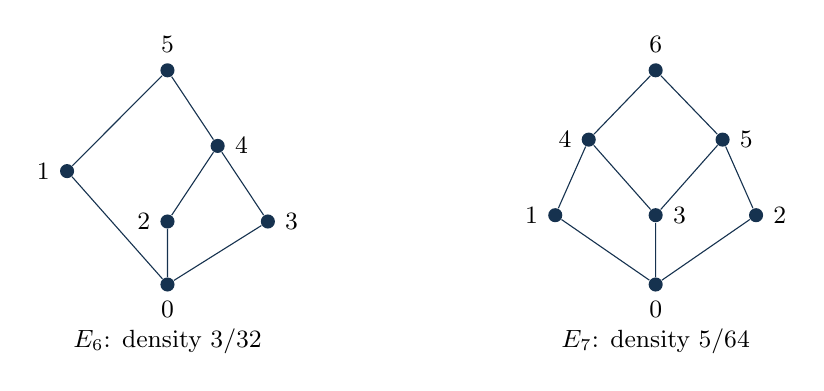
\begin{tikzpicture}[x=0.85cm,y=0.8cm,
  dot/.style={circle,fill=Ink,inner sep=1.8pt},every node/.style={font=\small}]
\begin{scope}[xshift=-3.1cm]
\node[dot,label=below:$0$] (z) at (0,0) {};
\node[dot,label=left:$1$] (a) at (-1.5,1.8) {};
\node[dot,label=left:$2$] (b) at (0,1) {};
\node[dot,label=right:$3$] (c) at (1.5,1) {};
\node[dot,label=right:$4$] (d) at (.75,2.2) {};
\node[dot,label=above:$5$] (t) at (0,3.4) {};
\draw[Ink] (z)--(a)--(t) (z)--(b)--(d)--(t) (z)--(c)--(d);
\node at (0,-.9) {$E_6$: density $3/32$};
\end{scope}
\begin{scope}[xshift=3.1cm]
\node[dot,label=below:$0$] (z) at (0,0) {};
\node[dot,label=left:$1$] (a) at (-1.5,1.1) {};
\node[dot,label=right:$2$] (b) at (1.5,1.1) {};
\node[dot,label=right:$3$] (c) at (0,1.1) {};
\node[dot,label=left:$4$] (d) at (-1,2.3) {};
\node[dot,label=right:$5$] (e) at (1,2.3) {};
\node[dot,label=above:$6$] (t) at (0,3.4) {};
\draw[Ink] (z)--(a)--(d)--(t) (z)--(b)--(e)--(t)
 (z)--(c)--(d) (c)--(e);
\node at (0,-.9) {$E_7$: density $5/64$};
\end{scope}
\end{tikzpicture}
\caption{Two illustrative nonextremal fans. On the left two fan labels coincide
and are smaller than the third. On the right all three labels are distinct,
but one is below both others.}
\label{fig:examples}
\end{figure}

\begin{table}[htbp]
\centering\small
\begin{tabular}{@{}lrrrrrrcc@{}}
\toprule
Lattice & $n$ & $k$ & $r$ & $m$ & $I(P)$ & $\card{\Con}$ & Density & Profile bound\\
\midrule
$M_2$ &4&2&2&1&4&4&$1/2$&$1/2$\\
$M_3$ &5&3&1&1&2&2&$1/8$&$1/8$\\
$M_4$ &6&4&1&1&2&2&$1/16$&$1/16$\\
$E_6$ &6&3&2&2&3&3&$3/32$&$3/32$\\
$E_7$ &7&3&3&3&5&5&$5/64$&$5/64$\\
$T_3$ &6&3&1&1&2&3&$3/32$&$1/8$\\
$B_3$ &8&3&3&4&8&8&$1/16$&$1/16$\\
$C_2\glue M_3\glue C_2$ &7&3&1&1&2&8&$1/8$&$1/8$\\
\bottomrule
\end{tabular}
\caption{Exact profiles at the designated bottom fan, or at the bottom of the
$M_3$ summand in the last row. Here $B_3$ means the Boolean lattice of all subsets
of a three-element set, so it has eight elements. The profile bound is the
right-hand side of~\eqref{eq:profile} for density.}
\label{tab:profiles}
\end{table}

For the Boolean lattice $B_d$ of all subsets of a $d$-element set,
$\Ji(B_d)$ consists of the singleton subsets. Its $d$ labels are independent:
for any collection of coordinates to forget, equality on all the other
coordinates is a congruence. Hence it has exactly $2^d$ congruences and
\[
 \cdens(B_d)=2^{d-2^d+1}.
\]
Its bottom has $d$ covers. This illustrates how much stronger the actual density
decay can be when many different labels create many join-reducible elements.

\subsection{Why two covers are exceptional}
For $k=1$, there is no improvement over density~$1$; chains attain it.
For $k=2$, the join of two distinct upper covers is join-reducible, so
$\cdens(L)\le1/2$ by~\eqref{eq:classical}. The four-element lattice $M_2$ attains
$1/2$, whereas $2^{-2}=1/4$. Thus the proposed formula is genuinely false for
two covers. In the proof of Lemma~\ref{lem:budget}, the missing ingredient is
exactly the third cover needed when $r=2$.

The sharp maximum densities under an ``at least $k$ covers'' constraint are
therefore $1$ for $k=1$, $1/2$ for $k=2$, and $2^{-k}$ for $k\ge3$, whenever the
specified size admits such a lattice. The minimum sizes are respectively
$2$, $4$, and $k+2$.

\section{A quadratic bound for the skeleton}\label{sec:skeleton}
We now use the established cover theorem in the structural framework of the
source. Following Cz\'edli~\cite[Section~5, equation~(5.1)]{czedli}, put
\begin{equation}\label{eq:skeleton}
\begin{split}
 \Skel(L)={}&\Jr(L)\cup\Mr(L)\\
 &{}\cup\bigcup_{x\in\Jr(L)}\LoCov_L(x)
 \cup\bigcup_{x\in\Mr(L)}\UpCov_L(x).
\end{split}
\end{equation}
Here $\LoCov_L(x)=\{y:y\prec x\}$ and
$\UpCov_L(x)=\{y:x\prec y\}$.
When nonempty, this set is a sublattice: joins and meets of comparable members
are already members, while the join of incomparable members is join-reducible
and their meet is meet-reducible. A chain has empty skeleton.

\begin{theorem}[Quadratic skeleton bound]\label{thm:skeleton}
Let $0<p\le1$, put
\begin{equation}\label{eq:tD}
 t=\left\lfloor\log_2(1/p)\right\rfloor,
 \qquad D=\max\{2,t\},
\end{equation}
and let $L$ be a finite lattice with $\cdens(L)\ge p$.
Then
\begin{equation}\label{eq:skeleton-bound}
 \card{\Skel(L)}\le2t(D+1)
   =2t\bigl(\max\{2,t\}+1\bigr).
\end{equation}
In fact, each of $\card{\Jr(L)}$ and $\card{\Mr(L)}$ is at most $t$, and every
element has at most $D$ upper covers and at most $D$ lower covers.
\end{theorem}
\begin{proof}
By~\eqref{eq:classical}, $\cdens(L)\le2^{-\card{\Jr(L)}}$.
Together with $\cdens(L)\ge p$, this yields $\card{\Jr(L)}\le t$.
Apply the same argument to the order dual for $\Mr(L)$.

Suppose an element has $d\ge3$ upper covers. Theorem~\ref{thm:main} gives
$p\le\cdens(L)\le2^{-d}$, hence $d\le t$. Counts of zero, one, or two covers
are already at most $D$. Duality gives the lower-cover bound.
Finally, count the union in~\eqref{eq:skeleton}, allowing overlaps:
\begin{align*}
 \card{\Skel(L)}
 &\le\sum_{x\in\Jr(L)}\bigl(1+\card{\LoCov_L(x)}\bigr)
    +\sum_{x\in\Mr(L)}\bigl(1+\card{\UpCov_L(x)}\bigr)\\
 &\le\bigl(\card{\Jr(L)}+\card{\Mr(L)}\bigr)(D+1)\\
 &\le2t(D+1).
\end{align*}
\end{proof}

Cz\'edli's earlier numerical estimate uses
\[
 k(p)=\lfloor\log_2(1/p)\rfloor+3,
 \qquad
 f(p)=2k(p)\bigl(R_{k(p)-1}(k(p))+1\bigr)
\]
and gives $\card{\Skel(L)}\le f(p)$ for $\cdens(L)\ge p$
\cite[Lemma~5.5]{czedli}.
Theorem~\ref{thm:skeleton} replaces this Ramsey-dependent quantity by
$O((\log(1/p))^2)$. It is a bound for exactly the same skeleton, not for a
newly defined smaller invariant.

\begin{table}[htbp]
\centering
\begin{tabular}{@{}rrrrrrr@{}}
\toprule
$t$ &0&1&2&3&4&10\\
\midrule
$D$ &2&2&2&3&4&10\\
Skeleton upper bound &0&6&12&24&40&220\\
\bottomrule
\end{tabular}
\caption{Values of the proved skeleton bound. The $t=0$ case says that density
strictly greater than $1/2$ forces a chain. The table gives upper bounds, not
claims that each is optimal.}
\end{table}

The theorem does not bound $\card L$ in terms of $p$.
Arbitrarily long chains have density~$1$, and adding exterior chains preserves
any lattice's density by the glued-sum formula.
The source's structural lemmas explain how skeletons encode branching while
chain segments can remain unbounded~\cite[Lemmas~5.2--5.4]{czedli}.
The quadratic estimate concerns that bounded branching part only.

\section{Exact computational verification}\label{sec:verification}
\subsection{Enumerating every small lattice without a database}
The verifier uses Python's standard library and integer arithmetic.
A \emph{natural labelling} of a poset on $\{0,\ldots,h-1\}$ means that
$x<_{P}y$ implies $x<y$ as integers. Such posets can be generated recursively:
after constructing the first $h$ vertices, the strict lower set of the new,
numerically largest vertex can be any order ideal of the existing poset.
Every natural poset is generated exactly once, because that lower set and the
induced old poset uniquely determine its final extension.

For $n\ge2$, the program enumerates natural posets on $n-2$ interior elements
and adds a bottom labelled~$0$ and a top labelled~$n-1$.
It retains precisely the orders in which every pair has a greatest lower bound
and a least upper bound. The singleton is treated separately.
Every finite lattice admits a natural labelling with these bottom and top
labels, by choosing a linear extension of its order. Therefore this process
includes every isomorphism class. It does \emph{not} eliminate isomorphic
natural labellings, and its counts must not be read as counts of isomorphism
classes.

Downsets and upsets are integer bitmasks. Meet and join tables, cover sets,
join-irreducibles, and the skeleton are computed from the order, not supplied
by a lattice database or inferred from a proposed family description.

\subsection{Two congruence computations}
The main computation obtains $\con(a,b)$ by starting with the equality relation,
merging $a,b$, and repeatedly closing under meet and join with every lattice
element. A union--find data structure maintains equivalence closure.
The process terminates because each effective merge reduces the number of
blocks. Every merge is forced in any congruence identifying $a,b$, and the final
partition is compatible; hence it is exactly the principal congruence.

All congruences are then generated as joins of the distinct labels $\gamma_j$.
The join is the equivalence closure of the union of two partitions.
Lemma~\ref{lem:signature} proves completeness of this generation method.
The program also directly checks the compatibility of every generated partition.

For every lattice of at most seven elements, a second computation enumerates
\emph{all set partitions} and tests compatibility directly, without using
principal labels or the generating theorem. The resulting sets of partitions
are compared for equality, not merely for equal cardinality.
This independently checks the congruence enumeration on 371 naturally labelled
lattices. Both methods are ordinary executable mathematics, not formal proofs
checked by a proof-assistant kernel.

\subsection{What was checked and what completed}
For each retained lattice, the program checks every selected subset of at least
three upper covers of every vertex. In particular, it checks fans that are
proper subsets of larger cover sets. For every such selection it verifies the
collision identities, $m\ge r$, the repeated-label exponent, the main bound,
the profile bound, the equality classification by direct order recognition,
and the nonextremal gap. It also checks the dual numerical bound and the
skeleton bound at the exact rational value $p=\cdens(L)$.

\begin{table}[htbp]
\centering\small
\begin{tabular}{@{}rrrrrrr@{}}
\toprule
$n$ & Interior posets & Lattices & Congruences & Fans & Equality fans & Second method\\
\midrule
1&1&1&1&0&0&1\\
2&1&1&2&0&0&1\\
3&1&1&4&0&0&1\\
4&2&2&12&0&0&2\\
5&7&7&49&1&1&7\\
6&40&39&281&17&3&39\\
7&357&320&2188&295&6&320\\
8&4824&3637&22743&5979&10&0\\
\midrule
Total & &4008&25280&6292&20&371\\
\bottomrule
\end{tabular}
\caption{Completed exhaustive verification. ``Congruences'' is the sum of
congruence counts over the naturally labelled lattices in that row.
``Second method'' counts lattices checked by all-partition enumeration.
For $n=1$, the interior-poset column uses the program's empty-interior convention.}
\label{tab:verification}
\end{table}

All checks in Table~\ref{tab:verification} passed.
Of the 6,292 fans, 1,137 have exactly two distinct labels and 108 have at least
three; thus the tests include the mixed-label cases essential to the argument,
not merely simple diamonds.
The maximum densities for fan sizes $3,4,5,6$ in the completed range are
$1/8,1/16,1/32,1/64$, respectively, as predicted.

Separately, the example program checks 35 structured cases: $M_k$ for
$3\le k\le20$; four diamond-with-chain examples; the one-edge subdivisions
$T_k$ for $3\le k\le12$; and the Boolean lattices $B_3,B_4,B_5$.
The last has 32 elements. These are selected larger examples, not an exhaustive
32-element enumeration. Their full-fan profiles and exact counts are in
\texttt{data/structured\_checks.json}.

The finite tests corroborate the arguments but do not replace them.
The all-$n$ statements depend on the written proofs. An exploratory run at
$n=9$ did not finish within the allotted tool time and is not included in the
completed scope or totals.

\subsection{Reproducing the archive}
From the archive's root directory, run
\begin{lstlisting}
python3 code/verify.py --max-n 8 --independent-through 7
python3 code/examples.py
latexmk -pdf -interaction=nonstopmode -halt-on-error sharp_cover_bound.tex
\end{lstlisting}
Python~3.10 or later is required for the type-annotation syntax; the recorded
run used Python~3.13. No numerical library, network connection, lattice database,
or external theorem prover is needed for verification.
The \LaTeX{} document uses standard AMS, Latin Modern, TikZ, and layout packages.
The recorded elapsed times are machine-dependent diagnostics; the mathematical
outputs use exact integers, partitions, and rational numbers.

The random-selection script is deliberately not part of the verification
command. Its recorded draw is an input to the project, not a theorem to be
regenerated. Re-running a genuinely random draw would not reproduce the same
outcome. The script refuses to overwrite the existing selection record.

\section{Proof audit and remaining scope}\label{sec:audit}
The main logical dependencies can be summarized without a computational step:
\[
 \text{transposition}
 \ \Longrightarrow\ \text{join collisions}
 \ \Longrightarrow\ m\ge r,
\]
\[
 \text{edge representatives}
 \ \Longrightarrow\ q\le n-1-m-k+r,
 \qquad
 \text{signatures}\ \Longrightarrow\ \card{\Con(L)}\le2^q.
\]
Combining the last two inequalities with $m\ge r$ proves the target.
The equality proof additionally uses antichain signatures and the elementary
quotient correspondence. The sharp gap uses the classical ideal representation.
The skeleton bound then follows by counting reducible elements and their covers.

Several possible pitfalls are avoided explicitly. The transposed upper interval
need not be prime. The fan representatives really are distinct even when their
labels coincide. A collision of disjoint pairs is handled separately from an
incident collision. The two-label case needs a repeated label and therefore a
third cover. The equality proof rules out additional elements inside the diamond
using quotient cardinality, not an unjustified assumption that a sublattice is
an interval. Finally, a skeleton bound is not a size bound for the whole lattice.

The proposed solution settles the stated all-$k$ implication within the argument
presented here. Independent specialist review would still be valuable,
particularly for the equality classification and priority assessment.
No claim is made of a Lean formalization, a new congruence-lattice representation
theorem, a full density-spectrum classification, or an optimal skeleton bound.

Two natural continuations remain. One is to improve the quadratic skeleton
estimate or to construct examples showing its correct asymptotic order.
The other is to characterize every lattice attaining the second constrained
value $3\cdot2^{n-k-3}$. The subdivision family proves that this value is sharp,
but the present argument does not assert that it exhausts the second-level
extremizers. A further multi-fan estimate would have to track shared labels;
one cannot simply multiply separate fan bounds without controlling their
dependence.

\appendix
\clearpage
\section{The random area selection}\label{app:selection}
The program used \texttt{secrets.randbelow(80)}, which obtains randomness from
the operating system. It returned the zero-based index~9, hence the one-based
index~10, \emph{lattice theory}. The ordered list below was fixed in the script
before the draw. Only one draw was made. The JSON record contains the list,
method, date, indices, selected area, and a zero redraw count.
It is a transparent execution record, not an independently certified random
experiment or a cryptographic commitment.

\begin{multicols}{2}
\small
\begin{enumerate}[leftmargin=2.6em,itemsep=0pt,parsep=0pt,topsep=0pt]
\item Finite group theory
\item Infinite group theory
\item Semigroup theory
\item Commutative algebra
\item Noncommutative algebra
\item Ring theory
\item Representation theory
\item Lie algebras
\item Universal algebra
\item \textbf{Lattice theory}
\item Order theory
\item Category theory
\item Type theory
\item Proof theory
\item Computability theory
\item Model theory
\item Set theory
\item Boolean algebras
\item Automata theory
\item Formal languages
\item Combinatorics on words
\item Symbolic dynamics
\item Topological dynamics
\item Ergodic theory
\item Discrete dynamical systems
\item Arithmetic dynamics
\item Elementary number theory
\item Additive number theory
\item Multiplicative number theory
\item Diophantine approximation
\item Diophantine equations
\item $p$-adic analysis
\item Finite fields
\item Coding theory
\item Design theory
\item Finite geometry
\item Matroid theory
\item Extremal graph theory
\item Algebraic graph theory
\item Spectral graph theory
\item Graph coloring
\item Graph domination
\item Graph enumeration
\item Hypergraph theory
\item Ramsey theory
\item Extremal set theory
\item Permutation patterns
\item Enumerative combinatorics
\item Algebraic combinatorics
\item Polyhedral combinatorics
\item Discrete geometry
\item Convex geometry
\item Combinatorial topology
\item Knot theory
\item Low-dimensional topology
\item General topology
\item Metric geometry
\item Fractal geometry
\item Real analysis
\item Complex analysis
\item Geometric function theory
\item Harmonic analysis
\item Functional analysis
\item Operator theory
\item Matrix analysis
\item Special functions
\item Orthogonal polynomials
\item Approximation theory
\item Asymptotic analysis
\item Analytic combinatorics
\item Generating functions
\item Integer sequences
\item Recurrence relations
\item Probability inequalities
\item Discrete probability
\item Random walks
\item Stochastic processes
\item Combinatorial game theory
\item Optimization
\item Numerical analysis
\end{enumerate}
\end{multicols}

\clearpage
\section{Compact verification algorithms}\label{app:algorithms}
The executable implementations are in \texttt{code/lattice\_tools.py}.
The following pseudocode displays the two essential closure procedures.
It deliberately does not enumerate ideals of a conjectured label order and then
assume that they are congruences.

\begin{lstlisting}
principal_congruence(L, a, b):
    P := the equality partition of L
    merge the blocks containing a and b
    repeat until no block changes:
        for x, y in the same block of P:
            for z in L:
                merge the blocks of meet(x,z) and meet(y,z)
                merge the blocks of join(x,z) and join(y,z)
    return P

all_congruences(L):
    labels := distinct principal_congruence(L, j_*, j)
              for all join-irreducibles j
    output := {equality partition}
    for gamma in labels:
        output := output union
                  {equivalence_closure(theta union gamma)
                   : theta in output}
    return output
\end{lstlisting}

The independent check instead generates every set partition $P$ and retains it
if, whenever $x,y$ share a block, the pairs
$x\wedge z,y\wedge z$ and $x\vee z,y\vee z$ share blocks for every $z$.
Testing one argument at a time suffices for compatibility in both arguments.

For equality recognition, the program does not use the number of congruences.
At the designated vertex $u$, it checks that there are exactly $k$ upper covers,
that all their pairwise joins are one vertex $v$, that every other vertex lies
below $u$ or above $v$, and that those two exterior intervals are chains.
This order-theoretic test is compared with numerical equality, so the equality
classification is not tested by a circular numerical definition.

\medskip
\noindent\textbf{Archive map.}
\texttt{sharp\_cover\_bound.tex} and \texttt{sharp\_cover\_bound.pdf} are the article.
\texttt{README.md} supplies commands and a result summary.
\texttt{STATUS.md} separates proved claims, executed tests, and unverified status.
\texttt{notes/} contains the source and proof audits.
\texttt{code/} contains the selection, enumeration, and example programs.
\texttt{data/} contains the original selection record, per-size verification
records, aggregate totals, worked examples, and structured larger checks.

\clearpage
\phantomsection
\addcontentsline{toc}{section}{References}
\begin{thebibliography}{9}
\bibitem{czedli}
G\'abor Cz\'edli,
\emph{Accumulation points of congruence densities of finite lattices},
version of 12 March 2026, 17 pp., arXiv:2603.11454v1.
\url{https://arxiv.org/abs/2603.11454}.
Target: Lemma~4.4 and the following sentence, p.~8.

\bibitem{freese}
Ralph Freese,
\emph{Computing congruence lattices of finite lattices},
Proceedings of the American Mathematical Society \textbf{125} (1997), no.~12,
3457--3463.
\url{https://doi.org/10.1090/S0002-9939-97-04332-3}.
Historical background; no result from this paper is used without a proof here.

\bibitem{czedli332}
G\'abor Cz\'edli,
\emph{Lattices with congruence densities larger than $3/32$},
author manuscript dated 28 July 2026; earlier version arXiv:2602.04321.
\url{https://arxiv.org/abs/2602.04321}.
Consulted author version:
\url{https://www.math.u-szeged.hu/~czedli/m/publ.pdf/czedli-cd-3-32.pdf}.

\bibitem{publist}
G\'abor Cz\'edli,
\emph{Publications}, author-maintained publication list,
entries 194--195, consulted 20 September 2026.
\url{https://www.math.u-szeged.hu/~czedli/m/listak/publist.html}.

\bibitem{manifest}
Vladimir Reshetnikov,
\emph{A manifest of docs/reports: seventy-one independent mathematical research
packages, classified by subject}, 20 September 2026.
User-supplied exclusion manifest, file \texttt{manifest(1).tex}.
Used only to avoid listed research targets; no result from it is assumed.
\end{thebibliography}
\end{document}
